\documentclass[12pt, a4paper, dutch]{article}
\usepackage[margin=1in]{geometry}

\usepackage{float}
\usepackage{babel}
\usepackage{siunitx}
\usepackage{amsmath}
\usepackage{csquotes}
\usepackage{parskip}
\usepackage{unicode-math}
\usepackage{fontspec}
\usepackage{tabularx}
\usepackage{booktabs}
\usepackage{needspace}
\usepackage{hyperref}
\usepackage{graphicx}
% \usepackage[backend=biber,
% 	bibencoding=utf8,
% 	style=apa
% ]{biblatex}

\setmainfont{TeX Gyre Schola}
\setmathfont{TeX Gyre Schola Math}
\sisetup{
	group-separator = {.},
	output-decimal-marker = {,}
}

\bigskipamount=7mm
\medskipamount=4mm
\parindent=0mm

\begin{document}
Ontwerpdocument \hfill \textbf{Loek Le Blansch (2180996)}\\
Project Stylofoon \hfill \today
\medskip

\section{Ontwerpschets}

\begin{figure}[H]
	\centering
	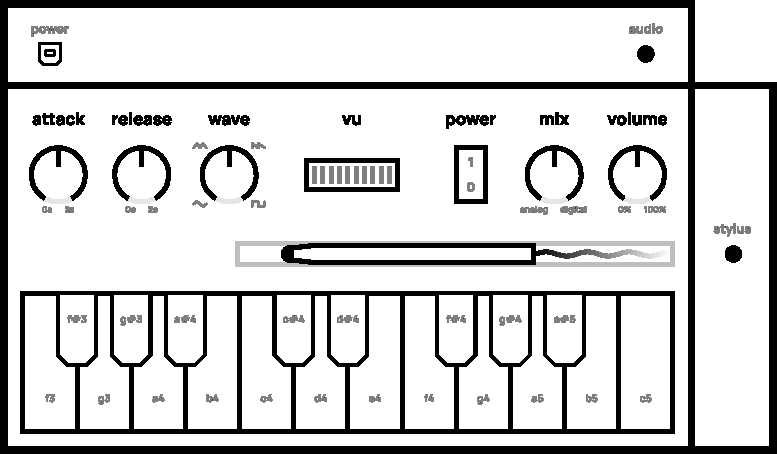
\includegraphics{figs/case-layout-sketch.pdf}
	\caption{Schets van de knoppenlayout op de voor-, zij- en bovenkant}
\end{figure}

\section{Blokschema}



\section{Elektrisch schema}
\section{PCB ontwerp}
\end{document}

